% ----------------------------------------
%
% LaTeX Article Template for CUED Reports
% Jon Sowman - 2009
% jon@hexoc.com
% 
% ----------------------------------------
% Set up the document class for an article
\documentclass[11pt]{article}

% Import the required packages for latex
\usepackage{appendix}

% This packages permits using $ \therefore $
\usepackage{amssymb}
\usepackage{graphicx}

% This package allows the use of $ \text{} $
\usepackage{amsmath}
\usepackage{savetrees}

% The document title and author
\title{SB3 - Datalogger\\Cambridge University Engineering Department} 
\author{David Turner \& Jon Sowman}

% Begin the document
\begin{document}
    \maketitle
	
% Insert the abstract for the document here
\begin{abstract}
    A compact, high speed logic analyser is designed with hardware buffering for the simultaneous analysis and logging of up to eight digital channels, one of which may be used as a synchronous clock, for analysis of asynchronous or synchronous digital communications. The supporting desktop application is also developed to configure and control the analyser, as well as to retrieve and post-process the recorded data and display it in a convenient format to aid debugging and analysis.
\end{abstract}

\section{Hardware Overview}
    A PIC18F4550 microcontroller forms the core of the data-logging hardware. The inbuilt USB peripheral is used along with support circuitry on the board for USB communications. A hardware reset function exists along with the option to run a bootloader, allowing the microcontroller to be programmed over the USB port.

    Additional hardware will be added to provide the following functionality:
    \begin{itemize}
    \item Provide input protection so moderate overvoltages do not damage the datalogger
    \item Log data from up to 8 digital channels, optionally synchronised to a clock on one channel
    \item Store up to 1Mbit of data (up to 128k samples with up to 8 digital channels per sample)
    \item Retrieve the samples from memory and transfer them to the desktop computer via the USB interface for post processing, analysis and charting
    \end{itemize}

    A schematic for the logic analyser hardware can be found in Appendix
    \ref{app-schematic}.

    \subsection{Filtering \& Conditioning}
    Frontend antialiasing filters will be put in place to avoid aliasing caused by input signals containing frequencies above the Nyquist frequency at which the device will sample. Simple first order low pass RC filters will suffice for this, with a $-3dB$ cut-off frequency placed just above the Nyquist frequency.

    Overvoltage protection is provided by eight operational amplifiers
    configured as inverting comparators with the threshold voltage set as
    Vcc/2. These amplifiers can tolerate inputs of up to 32V without damage, and
    will prevent this voltage being passed on to the octal buffer where it could
    cause damage.

    The disadvantage of using these amplifiers is that the Schmitt trigger type inputs on the MCU will have no effect, so the protection amplifiers will be
    configured with some hysteresis to reintroduce the added noise immunity.

\subsection{Buffering}
    The data will be captured directly by an SRAM (Static Random Access Memory) buffer during the logging process, since the PIC does not have enough internal RAM to store enough samples to satisfy the specification. SRAM, whilst relatively expensive, is capable of very fast write speeds, essential to achieve a high sampling rate.

    The memory chosen is the AS6C1008 1Mbit SRAM IC from Alliance Memory. A 17-bit wide parallel interface is used for byte-addressing and an 8-bit parallel interface is used for data.

    The address lines will be directly attached to the PIC using the two byte-wide ports PORTB and PORTD, plus one additional line from another port. After the hardware anti-aliasing filters, the eight input channels are connected via a shared data bus to the SRAM data interface via a 8-way tri-state buffer, controlled by the PIC. This buffer is enabled during the data acquisition phase, and subsequently disabled when the PIC reads back the data from the SRAM.

    Synchronous data capture is possible using the clock input line, which allows one input line to bypass the shift register and be connected directly to the PIC.  The PIC will interrupt on changes of this line and capture data to the SRAM on the appropriate clock edge (set by the user).

\subsection{Data Retrieval}
    Retrieving data from the SRAM is achieved via the use of a parallel-in/serial-out shift register such as the 74HC165 series in order to reduce the number of IO pins required on the microcontroller. The byte-wide parallel input to this device is attached to the data bus, and data is clocked in to the PIC before being packetised and transmitted to the desktop computer over the USB interface.

    A block diagram of the hardware of the data capture system is shown in figure \ref{fig:app}.
    
\subsection{Software Interface}
    The software interface will be developed using the LabWindows environment and will allow configuration and initiation of datalogging and viewing and analysis of captured data.  The user can select either the asyncronous sample rate or synchronous mode, which channels to capture, and number of samples to capture.  The software will have options to immediately initiate the capture, wait for a trigger byte on the 8 channels, or begin capture on a rising or falling edge of the clock line.  Once the capture is complete and data has been streamed to the PC, it will be available for viewing in both timing diagram and listing forms, with optional ASCII interpretation of the listing.

\section{Firmware}
\subsection{Command Response Protocol}
    The MCU firmware will be event driven according to a command/response
    specification. Command bytes followed by a payload will be received from the
    PC, in the following format: \\

    \texttt{[CMD, LEN, D0, D1,  ...]} \\

    Where D are data bits, up to 62 permitted per packet. Data is returned
    to the PC from the MCU in a similar manner. \texttt{LEN} is the total number
    of bytes in the packet, including the \texttt{CMD} and \texttt{LEN} bytes.

\subsection{Data Acquisition}
    To begin datalogging, a configuration command (\texttt{CFG}) 
    is first sent to the analyser
    to set all configurable options, which would otherwise be a in default power
    up state. These options include sample rate and synchronous or asynchronous
    modes.

    An \texttt{ARM} command is then sent to the analyser, which will either wait
    for a change on channel 1 (clock) (in synchronous mode) or begin logging
    immediately (in asynchronous mode). The analyser will confirm beginning
    sampling by returning a START (\texttt{SRT}) packet to the PC, which 
    will then
    wait until an \texttt{END} command is received signalling the end of
    sampling. The PC will be able to cancel the logging by sending a CANCEL
    (\texttt{CNL}) command at any point during the logging process. During
    logging, the MCU will clock data into SRAM at the sample rate given, or on
    the rising/falling (configurable) edge of channel 1 (clock).

\subsection{Data Recovery}
    The PC will know when sampling has completed and can then request the sample
    data from the analyser. The MCU will confirm the start of data recovery, and
    then proceed to packetise the samples into 64 byte packets, which includes
    the \texttt{CMD} and \texttt{LEN} fields. These packets are transmitted over
    the USB interface until the SRAM is empty, with termination by a
    \texttt{END} command packet. Data is lost from the volatile SRAM on power
    removal, so data recovery must be completed before the unit is powered down.

\section{Software}
    Waffle about the PC side software and GUI, plus a block diagram.
    
    \begin{figure}
    \centering
    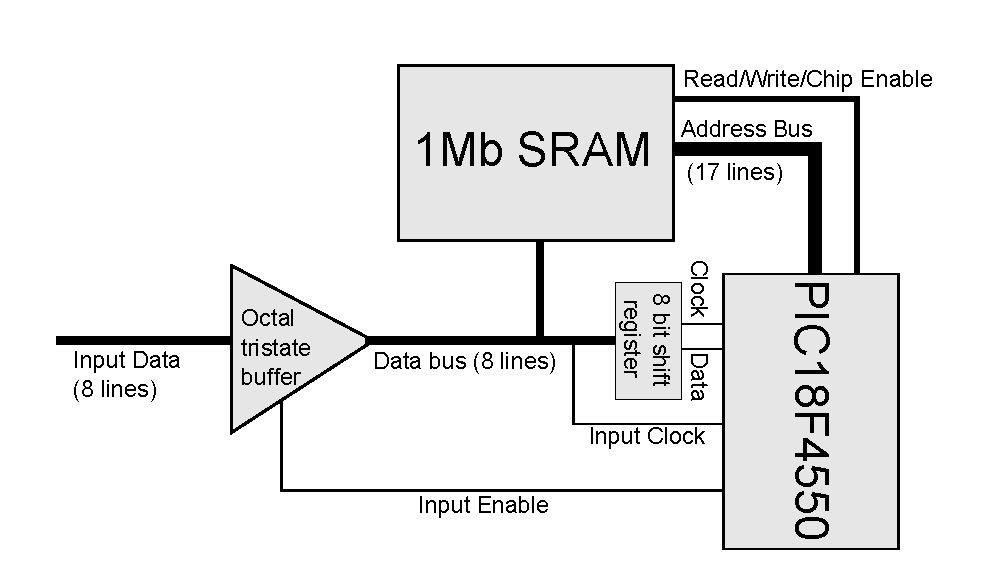
\includegraphics[height=8cm]{hardware.pdf}
    \caption{Capture Hardware}
    \label{fig:app}
    \end{figure}

    \begin{figure}
    \centering
    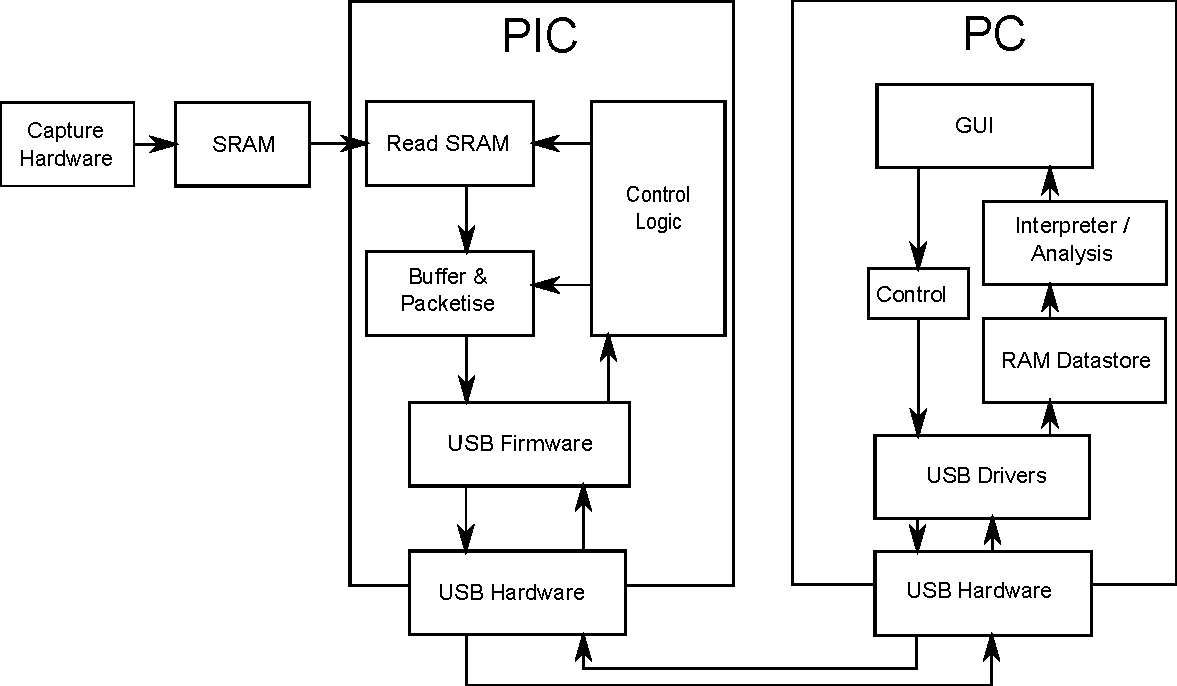
\includegraphics[height=8cm]{block-diagram.pdf}
    \caption{System Block Diagram}
    \label{fig:app}
    \end{figure}
	
% Now print the appendix section
\appendix
\appendixpage
\addappheadtotoc
\section{Schematic}
\label{app-schematic}
			
    \begin{figure}
    \centering
    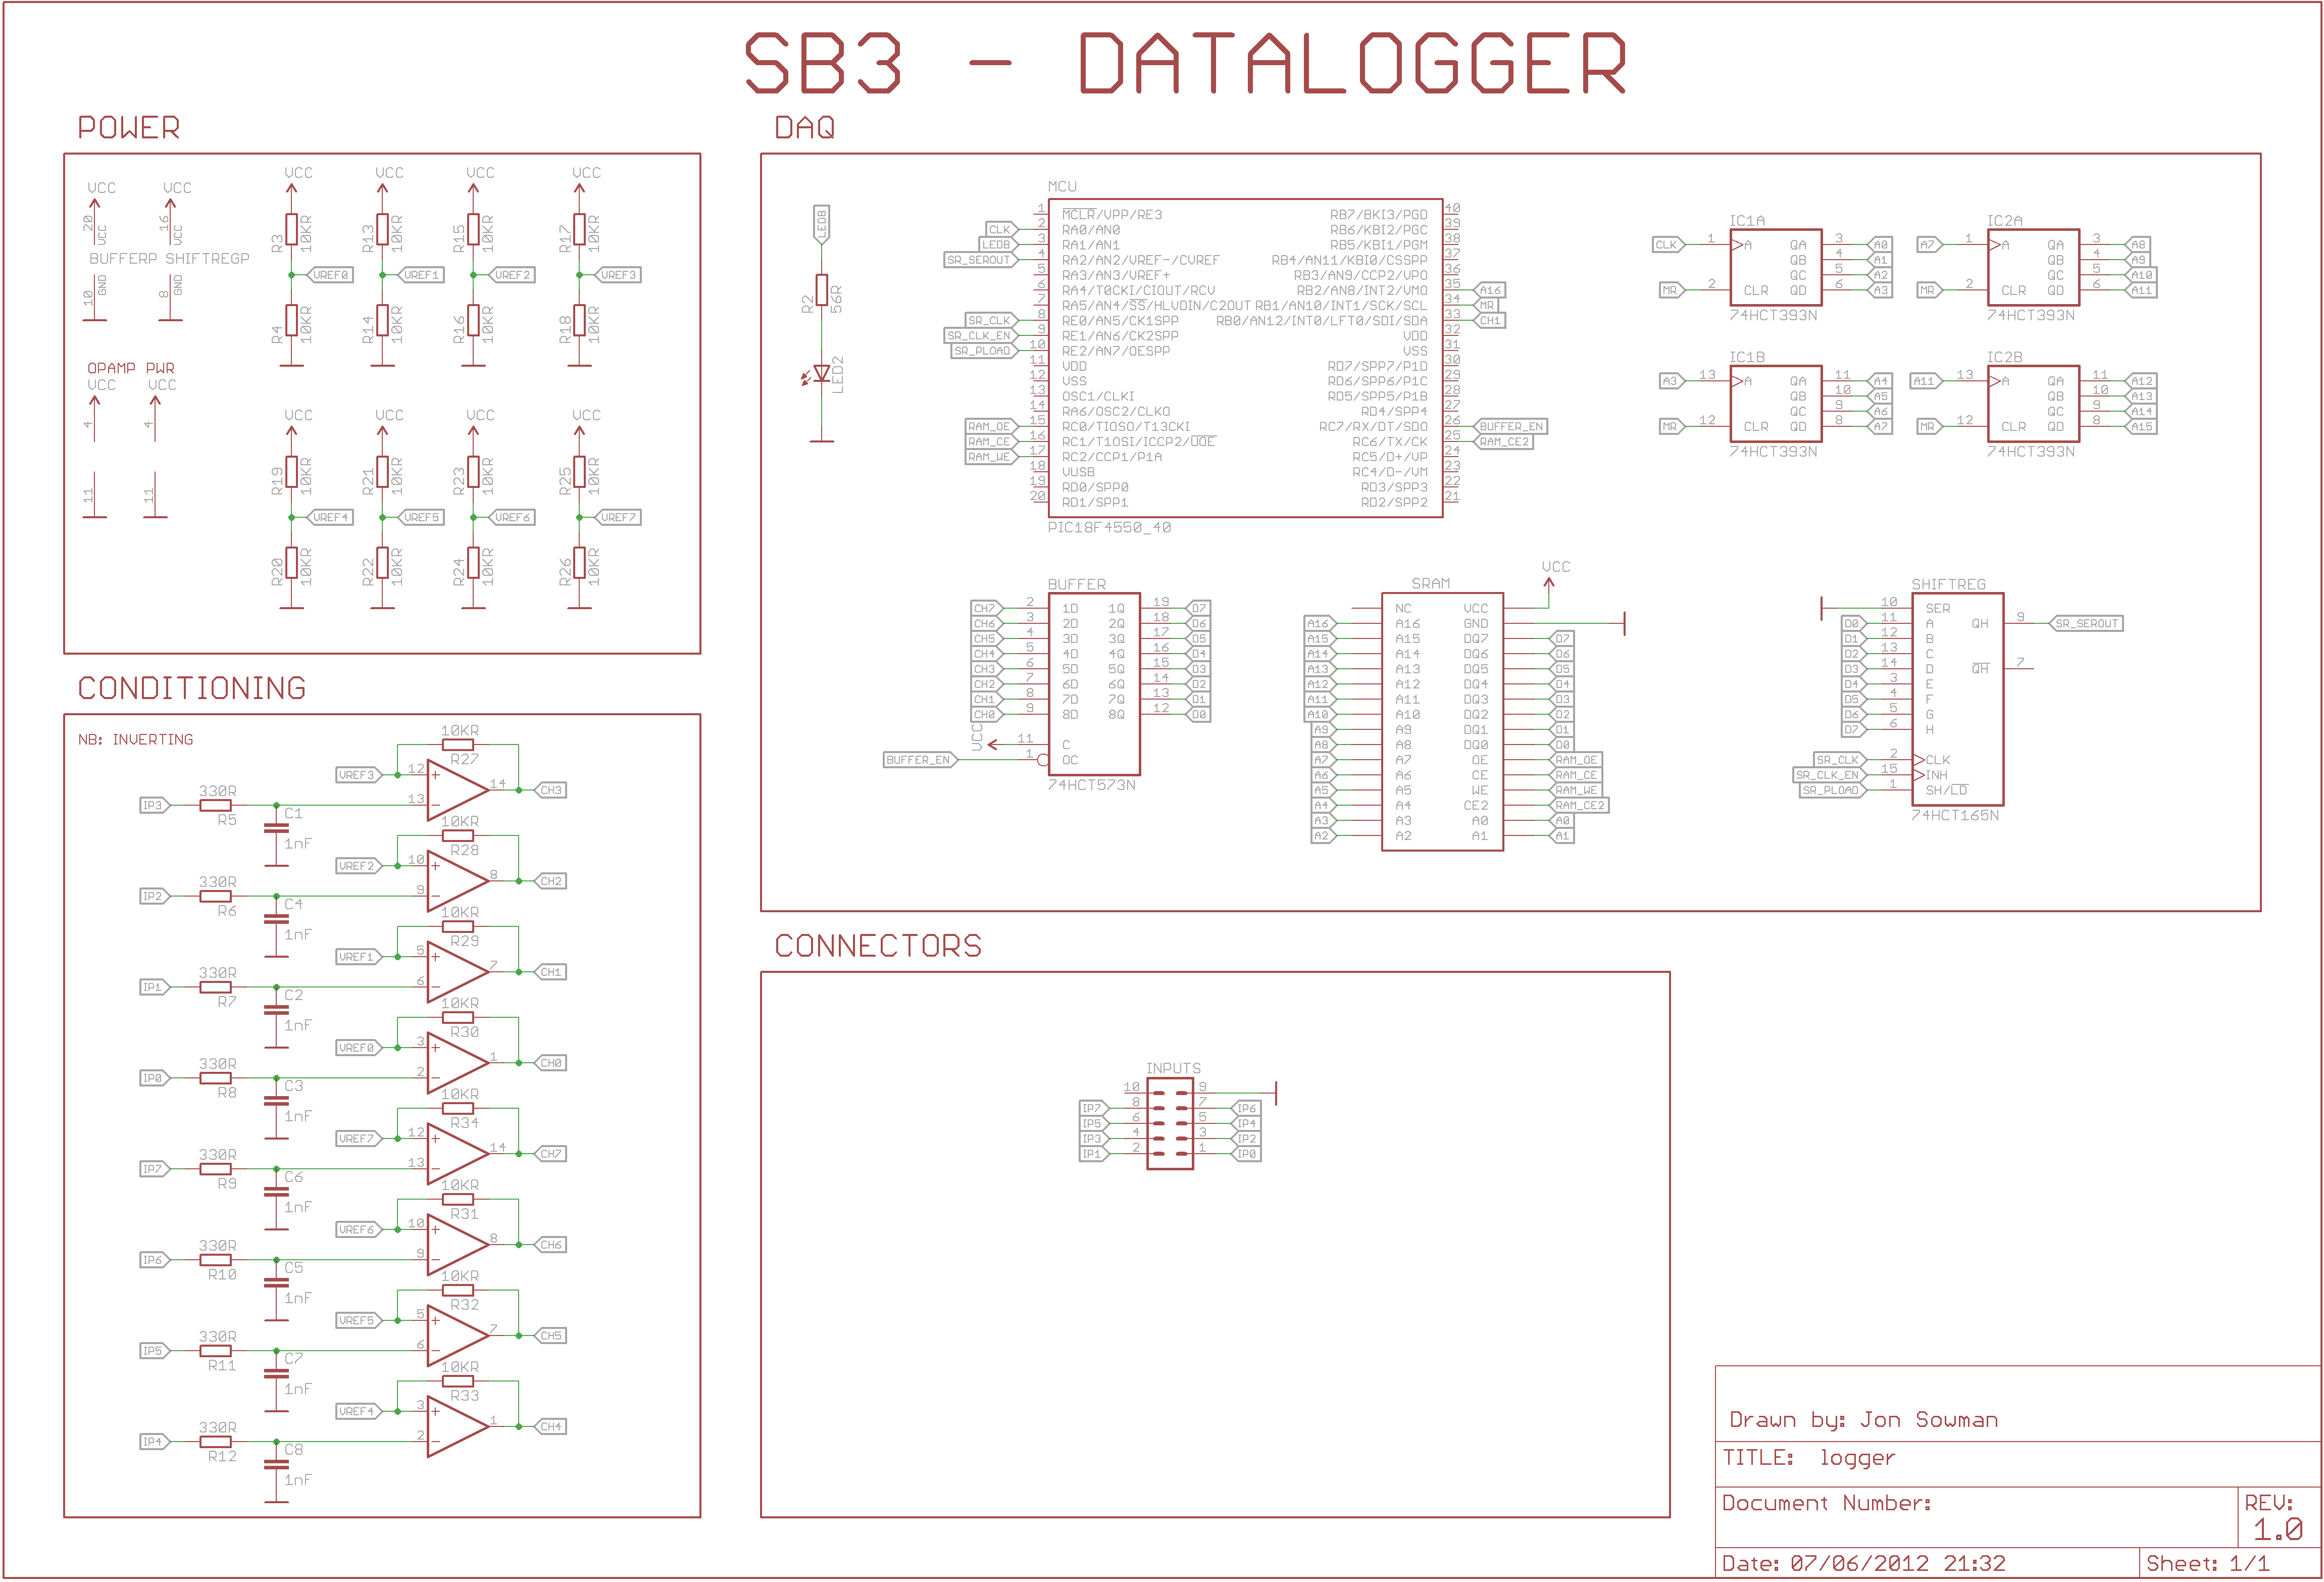
\includegraphics[height=17cm,angle=90]{../../hardware/schematic.png}
    \caption{Logic analyser schematic}
    \label{fig:sch}
    \end{figure}

\section{Bill of Materials}
    All parts are from Farnell Onecall and prices are list, pre-discount.

    \begin{table}
    \begin{center}
    \begin{tabular}{|r|c|c|c|}
        \hline \textbf{Part No.} & \textbf{Description} & \textbf{Qty} & \textbf{Price/£ }  \\
        \hline 380365 & 74HC165 PISO Shift Register & 1 & 0.38 \\
        \hline 1562896 & Alliance 1Mbit SRAM & 1 & 2.44 \\
         \hline 382449 & 74HCT573 Octal Latch & 1 & 0.58 \\
        \hline 1750143 & Quad Operational Amplifier & 2 & 0.15 \\
        \hline 1841236 & SIL 0.1" 32-way header & 1 & 1.88 \\
        \hline 1667501 & SIL 0.1" 32-way socket & 1 & 3.82 \\
        \hline
    \end{tabular}
    \end{center}
    \caption{Bill of materials for the logic analyser}
    \label{fig:myt}
    \end{table}
	
\end{document}
